\chapter{Young Entrepreneur Interviews Shaq}

This lecture is built like a compressed field manual. It begins by spending its conclusions before it spends its explanations, then resets, then returns to the same claims in slower and more usable form. What emerges is not a theory of wealth in the abstract, but a sequence of operator rules: scale by delegation, learn by patterned imitation, distinguish making money from keeping it, price from strength, hire above oneself, and treat motivation as a form of durable energy rather than a passing mood. The mathematics here is light but real. It appears as counts, ratios, bargaining ladders, retention rules, and asymmetries, and those are exactly the places where the transcript becomes most teachable.

\section{Cold Open and the Atlanta Reset}

The lecture first arrives as a teaser reel. We hear the name, the many-industry identity, the old fact of owning \(155\) Five Guys locations, the single word ``delegation,'' the claim of coming from no money, the motivation of being able to give his mother what she wants, the affirmation of faith, the moment of spontaneous generosity with pizza, and then the unanswered question about the most money made in a single year. The structure matters. We are not yet being taught in sequence. We are being shown the theorem list before the proof.

Only after that does the host reset the scene in Atlanta and tell us what sort of lesson this is supposed to be. Shaq is framed as one of the greatest athletes in the history of the NBA and also as a business mogul with hundreds of businesses around the country. The rough wealth marker is also inserted here, though in slightly garbled form, as a net worth near \(\text{\$}500\) million. That number is host-side framing rather than Shaq's own doctrine, but it sets the scale of the investigation.

What the reset really does is convert celebrity into method. We are no longer merely being asked who Shaq is. We are being asked what kind of rules one must learn to move from performance to scale, and from income to retained wealth.

\section{Delegation and the Arithmetic of Scale}

The first crisp business principle in the lecture comes from a number:
\begin{equation}
N_{\text{FG}} = 155.
\end{equation}
The host brings up the old Five Guys position, and Shaq answers the scaling question with one word: delegation. The explanation is arithmetically simple and operationally decisive. One person cannot be present in \(155\) places at once. Therefore direct personal presence is not the mechanism of scale.

We can write the logic in its minimal form as
\begin{equation}
1\ \text{owner} \not\Rightarrow N_{\text{FG}}\ \text{locations run directly},
\end{equation}
and then in the positive direction as
\begin{equation}
\text{delegation} \Rightarrow \text{parallel operators} \Rightarrow \text{scale}.
\end{equation}
This is not a formal theorem from management science; it is the transcript's own compression of the problem. The point is not merely that delegation is helpful. The point is that once the count becomes large enough, delegation stops being optional and becomes the operating form of the business.

\begin{figure}[h]
\centering
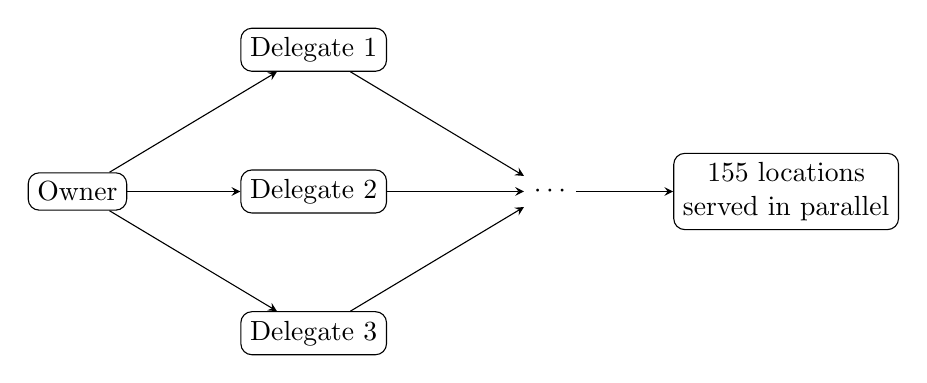
\begin{tikzpicture}[>=stealth]
\node[draw,rounded corners,align=center] (owner) at (0,0) {Owner};
\node[draw,rounded corners,align=center] (d1) at (3,1.8) {Delegate 1};
\node[draw,rounded corners,align=center] (d2) at (3,0) {Delegate 2};
\node[draw,rounded corners,align=center] (d3) at (3,-1.8) {Delegate 3};
\node[align=center] (dots) at (6,0) {\(\cdots\)};
\node[draw,rounded corners,align=center] (loc) at (9,0) {155 locations\\served in parallel};

\draw[->] (owner) -- (d1);
\draw[->] (owner) -- (d2);
\draw[->] (owner) -- (d3);
\draw[->] (d1) -- (dots);
\draw[->] (d2) -- (dots);
\draw[->] (d3) -- (dots);
\draw[->] (dots) -- (loc);
\end{tikzpicture}
\caption{Transcript-based reconstruction of the lecture's core scaling claim: scale comes from delegated parallelism rather than from the owner's personal presence.}
\end{figure}

Later in the lecture this same principle returns through the language of championships and teammates. That return is important. Delegation is not presented as an office technique alone. It is part of a larger habit of winning through strong others.

\subsection{Question \& Answer}

\paragraph{Question.} How do we scale when one person cannot physically occupy \(155\) locations at once?

\paragraph{Answer.} The lecture's answer is not to work harder, travel faster, or centralize more tightly. The answer is to replace direct presence with trusted distributed execution. In transcript language, that replacement is called delegation. In note form, it is the passage from singular control to parallel operators.

\section{Stealing Greatness Without Becoming a Copy}

The most arresting line in the lecture is not numerical but structural. When asked about the biggest driving factor behind his success, Shaq answers, ``I was a thief,'' and then immediately adds, ``Let me explain.'' The explanation matters enough to preserve with some notation.

The named source set is
\begin{equation}
\mathcal{E}=\{\text{Jordan},\text{Magic},\text{Kareem},\text{Ali}\}.
\end{equation}
He says that if one sees somebody doing better and wishes to aspire upward, one should steal what they are doing. For him this means not copying one person whole, but taking selected elements from several exemplars and placing them ``inside'' the mind. The lecture's implied transformation is therefore
\begin{equation}
\mathcal{E} \to \text{internal synthesis} \to \text{constructed self}.
\end{equation}

This is one of the strongest conceptual moments in the interview because it refuses two weak alternatives. It refuses the myth of pure originality, and it also refuses the passivity of imitation as mere duplication. What is borrowed are methods, energies, and forms of excellence. What is produced at the far end is still a singular operator.

\subsection{Question \& Answer}

\paragraph{Question.} What does Shaq mean by ``steal what they are doing,'' and how does imitation become authorship rather than mere copying?

\paragraph{Answer.} The lecture resolves the tension by making the theft selective and synthetic. One does not become Jordan, Magic, Kareem, or Ali. One studies them, extracts working traits, combines them, and then creates oneself. The point is not plagiarism of identity. It is intelligent borrowing under pressure.

\section{Making Money, Losing Money, Keeping Money}

From success the lecture moves to a harsher question: how does one keep large wealth once it arrives? The host introduces a speaker-cited statistic:
\begin{align}
p_{\text{broke,NFL}} &\approx \frac{1}{3}, &
t_{\text{post-career}} &\approx 3\text{--}5\ \text{years}.
\end{align}
The immediate lesson is an asymmetry:
\begin{equation}
\text{easy to make a lot of money} \neq \text{easy to keep a lot of money}.
\end{equation}
This is not merely a slogan. It is the governing distinction of the middle of the lecture. Earning and retaining are two different problems, and the interview insists that many people confuse them until it is too late.

Shaq then gives a single financial term rather than a full lecture:
\begin{equation}
\text{preservation keyword} = \text{annuity}.
\end{equation}
But the transcript is equally important for what it does \emph{not} do. He refuses to unpack the term, tells the audience to look it up, and does not turn the interview into a finance seminar. The chapter should preserve that restraint. The word matters because it marks financial literacy as a threshold, not because the lecture derives annuity formulas on the page.

The later autobiographical material clarifies the point more vividly than a definition would. The first million dollars, he says, disappeared in roughly half an hour:
\begin{equation}
\text{\$}1{,}000{,}000 \to \text{spent in about }30\ \text{minutes}.
\end{equation}
The story is not there for comic color. It is there to show how rapidly cash can dissipate when scale arrives before structure.

\subsection{Question \& Answer}

\paragraph{Question.} Why is keeping money harder than making money once large income arrives quickly?

\paragraph{Answer.} Because the arrival of money does not automatically bring along the habits, structures, and vocabulary needed to preserve it. The lecture's own evidence is double: a public statistic about athlete bankruptcy and a private confession about spending a first million almost immediately. Wealth retention is therefore a second education layered on top of wealth acquisition.

\section{The Interrupted Middle and the Return to Operator Rules}

At precisely the point where the interview is about to press on business count and annual revenue, the lecture is interrupted by a long host-side detour about mentorship, access, and community. This break is part of the source and should not be erased, but it should also not be mistaken for Shaq's own doctrine. The interruption carries its own scale markers,
\begin{align}
V_{\text{Hilton sale}} &= \text{\$}2.2\ \text{billion}, &
F_{\text{channel}} &> 10\ \text{million},
\end{align}
yet these numbers belong to the channel's self-positioning rather than to the internal logic of Shaq's answer set.

When the lecture returns to Shaq, the tone changes. Peak-year money does not interest him much; he says he does not do things for monetary purposes and does not even know the exact amount of money he has in today's world. Instead the lecture turns toward reusable operator heuristics.

First comes the distinction between starting something from inspiration and copying something already working. That claim is immediately paired with a failure-rate heuristic:
\begin{align}
p_{\text{firm failure}} &\approx \frac{8}{10}, &
t_{\text{firm failure}} &\approx 5\ \text{years}.
\end{align}
The lesson is not that invention is impossible. It is that uncertainty is expensive, and visible working demand is evidence one should not ignore.

Second comes the advice to hire people smarter than oneself. This belongs with delegation, but it sharpens it. Delegation is not merely about distributing tasks. It is also about accepting superior competence elsewhere.

Third comes the retention rule from a mentor:
\begin{equation}
s = 0.75Y,\qquad c = 0.25Y,\qquad s+c=Y.
\end{equation}
Here \(Y\) is income, \(s\) the saved share, and \(c\) the share used for enjoyment. The rule is crude, but the lecture values it precisely because it is memorable enough to survive contact with real money.

Finally, the interview turns numerical in a much more explicit way through negotiation. Shaq says not to talk first and to start high. The bargaining ladder is given as
\begin{align}
a_0&=200, &
a_1&=110, &
a_2&=140, &
a_3&=125,
\end{align}
or, more narratively,
\begin{equation}
200 \to 110 \to 140 \to 125 \to \text{deal}.
\end{equation}
We may write the worked example exactly as the lecture means it. If the other side can spend
\begin{equation}
B=200,
\end{equation}
and we open at
\begin{equation}
a_0=50,
\end{equation}
then the immediately surrendered room is
\begin{equation}
B-a_0 = 200-50 = 150.
\end{equation}

\paragraph{Worked example.}
\begin{enumerate}
\item Take the other side's budget to be \(B=200\).
\item Suppose the opening ask is only \(a_0=50\).
\item Then the negotiable room given away at the start is \(B-a_0\).
\item Numerically, this is \(200-50=150\).
\item The lecture's conclusion is that a weak opening destroys surplus before the negotiation has even begun.
\end{enumerate}

\subsection{Question \& Answer}

\paragraph{Question.} Why does Shaq insist that we should not talk first and should start high?

\paragraph{Answer.} Because the opening number is not just a sentence; it is an anchor. The lecture's own arithmetic shows that if the counterparty's budget is much higher than the first ask, then the difference is not hypothetical. It is bargaining room surrendered in advance. The point is not theatrical aggression. It is preservation of negotiating space.

\section{Motivation, Risk, and the Final Blueprint}

The lecture now loops back through biography in order to justify its earlier principles. Delegation returns, but now in the language of championships and teammates. That return matters: what worked in competitive sport becomes a model for business structure. Then the personal history enters more directly. There was no inherited money. There were horror stories about athletes going broke. There was financial ignorance, including not knowing what FICO meant. There was also the now-famous first-million mistake. The rules are therefore presented not as polished abstractions but as corrections learned under pressure.

The longevity question produces another numerical anchor:
\begin{equation}
t_{\text{NBA}} = 19\ \text{years}.
\end{equation}
The answer is again motivational. At first the engine was the desire to give his mother what she wanted. Later, once that need was satisfied, the energy had to come from somewhere else. The lecture does not formalize that second source, but it does preserve the key point: durable performance requires durable motive.

Faith then enters not as ornament but as grounding. Immediately after that comes one of the lecture's strongest business regrets: not taking the Starbucks opportunity because he misunderstood the economic transformation of neighborhoods. The relevant count is given cautiously as
\begin{equation}
N_{\text{Magic Starbucks}} \approx 155.
\end{equation}
The error here is not laziness but misreading context. A business opportunity was visible, but its true environment was not yet legible to him.

The late part of the lecture gathers several filters into a final operator profile. The most successful people, Shaq says, are nice, humble, simple, and surrounded by great people. Jeff Bezos becomes the source of an investment filter: invest in things that change people's lives. The pizza episode returns again to make ownership tangible. Asked what he looks for in founders, Shaq answers not with spreadsheets but with belief: he wants to believe in what they believe in. Asked how he found the self-belief to make hundreds of millions, he partially withdraws and attributes much to luck, citing the athletic advantage that gave him capital to leverage.

That hesitation is important. The lecture does not close by claiming that everything can be reproduced mechanically. It closes by mixing luck with method, which makes the final blueprint more credible rather than less. The closing advice can be compressed into a transcript-faithful chain:
\begin{equation}
\text{plan} \to \text{watch what works} \to \text{borrow} \to \text{add style} \to \text{persist}.
\end{equation}
And the lecture gives the same rule in imperative form:
\begin{enumerate}
\item write the plan down,
\item figure it out,
\item if someone is already doing it, watch them,
\item steal what works,
\item add one's own razzmatazz,
\item believe through the ups and downs.
\end{enumerate}

\subsection{Question \& Answer}

\paragraph{Question.} If luck mattered in Shaq's case, what part of the lecture still survives as general method?

\paragraph{Answer.} The lecture leaves us with a strong remainder even after luck is admitted. Delegation, hiring above oneself, saving before spending, anchoring high in negotiation, studying successful exemplars, recognizing working demand, writing the plan down, and persisting through volatility all survive the subtraction of luck. Luck may change the speed or scale of the outcome, but the method still governs the path.

\section{Summary}

This chapter is built from a lecture that thinks in counts, ratios, anchors, and asymmetries. The count \(155\) turns scale into a problem of structure. The set \(\mathcal{E}\) turns greatness into selective borrowing. The statistic \(\frac13\) over \(3\text{--}5\) years turns wealth into a preservation problem. The split \(75/25\) turns income into retained and consumed portions. The negotiation ladder \(200 \to 110 \to 140 \to 125\) turns bargaining into visible arithmetic. Around those numbers the lecture places its deeper constants: motivation, humility, strong people, belief, and the willingness to learn from both models and mistakes. The result is not a complete theory of wealth, but it is a sharp operating grammar for how wealth is made, structured, defended, and extended.